\documentclass{beamer}

%%%%%%%%%%%%%Solarized Theme%%%%%%%%%%%%%%%
\usecolortheme[dark,accent=cyan]{solarized}
\beamertemplatenavigationsymbolsempty
%%%%%Packages%%%%%
\usefonttheme{serif}
\usepackage[T1]{fontenc}
\usepackage[utf8]{inputenc}
\usepackage[english]{babel}
\usepackage{fontawesome}
\usepackage{minted}
\usepackage{soul}

\definecolor{DarkGray}{gray}{0.1}
\usemintedstyle{paraiso-dark}


\usepackage{graphicx}
\usepackage{hyperref}
\usepackage{colortbl, xcolor}
\usepackage{booktabs}
\usepackage{amsmath,amsthm, amssymb, latexsym}

\usepackage{tikz}
\usepackage{xcolor}
\usepackage{graphicx,multirow}
\definecolor{plain}{rgb}{93,93,93}
\usetikzlibrary{positioning,arrows}
\definecolor{applegreen}{rgb}{0.55, 0.71, 0.0}
\usetikzlibrary{decorations.pathreplacing, backgrounds, fit}
\usetikzlibrary{calc,matrix}
\usepackage{relsize}
\tikzset{fontscale/.style = {font=\relsize{#1}}
    }

\tikzstyle{background}=[solarizedRed, rectangle, draw, inner sep=1mm, thick,
           rounded corners=2mm]

\usepackage{standalone}
\usepackage{siunitx}

\begin{document}

\begin{frame}
    \begin{center}
        \large{\textsc{Homophily and minority-group size explain perception biases in social networks}} \\

        \vspace{1cm}
        \footnotesize{Eun Lee, Fariba Karimi, Claudia Wagner, Hang-Hyun Jo, Markus Strohmaier \& Mirta Galesic}

    \end{center}
\end{frame}

\begin{frame}
    \begin{center}
        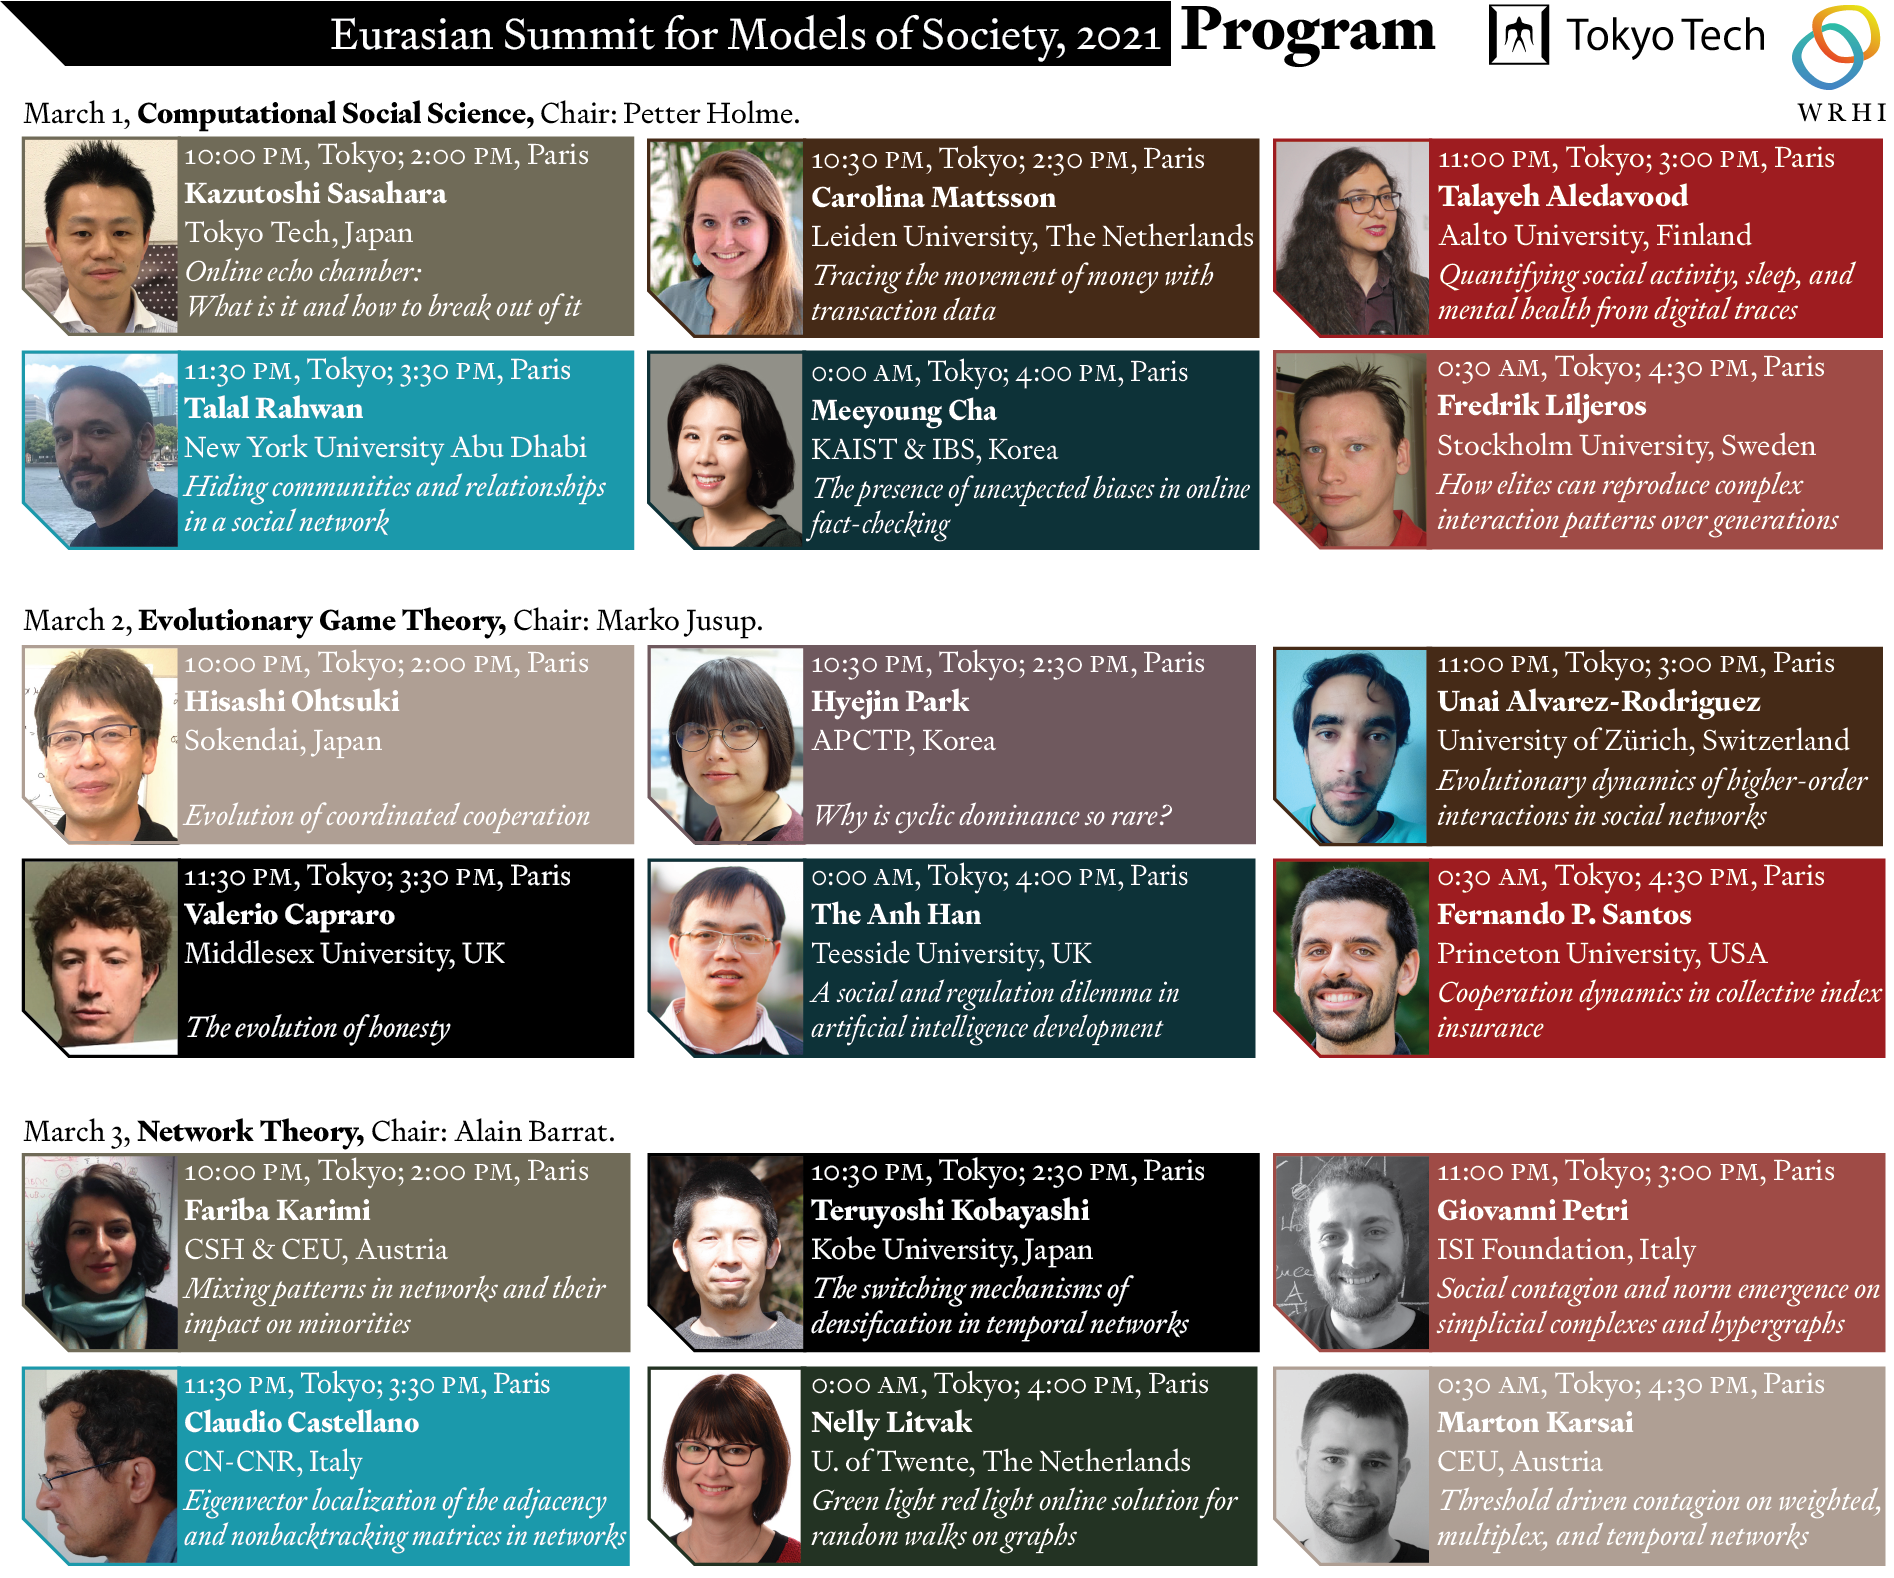
\includegraphics[width=\textwidth]{static/eurasian_summit.png}
    \end{center}
\end{frame}

\begin{frame}
    \begin{center}
    \begin{minipage}{.5\textwidth}
        \LARGE{MINORITY}
    \end{minipage}
    \begin{minipage}{.3\textwidth}
        \normalsize{[mai - no - ruh - tee]}
    \end{minipage}
    \vspace{.5cm}

    \hspace{-8cm} \normalsize{[noun]}\\
    \end{center}
    \hspace{.8cm} \normalsize{1. the smaller number or part, especially a number or part} \\
    \hspace{.8cm} \normalsize{representing less than half of the whole.}
\end{frame}

\begin{frame}
    \begin{center}
        
\includegraphics[width=\textwidth]{static/stem.jpg}
    \end{center}
\end{frame}

\begin{frame}
    \begin{center}
    \begin{minipage}{.5\textwidth}
        \LARGE{HOMOPHILY}
    \end{minipage}
    \begin{minipage}{.3\textwidth}
        \normalsize{[huh - mof - uh - lee]}
    \end{minipage}
    \vspace{.5cm}

    \hspace{-8cm} \normalsize{[noun]}\\
    \end{center}
    \hspace{.8cm} \normalsize{1. the tendency to form strong social connections
    with people who share one’s defining characteristics, as age, gender, ethnicity, 
    socioeconomic status, personal beliefs, etc.:}
\end{frame}

\begin{frame}
    \begin{center}
        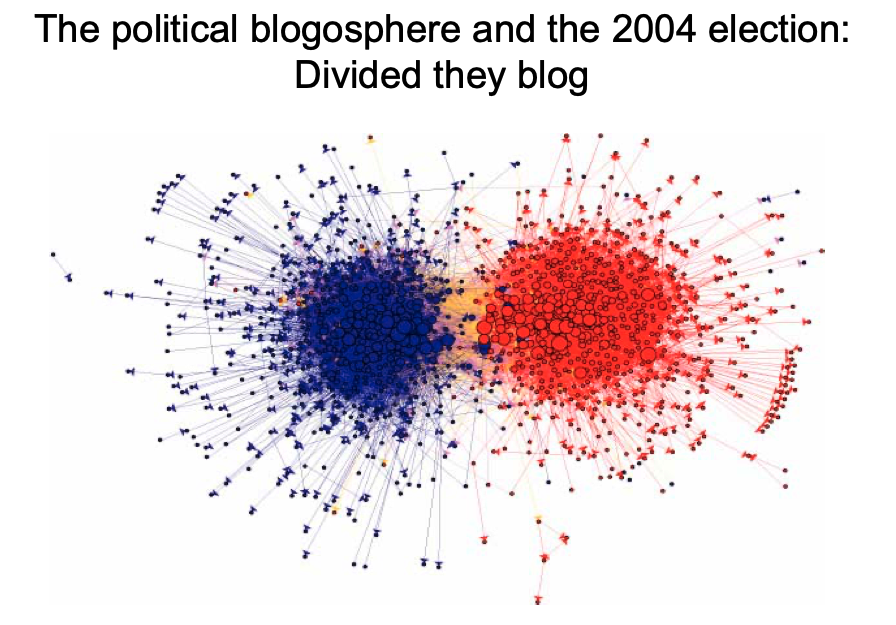
\includegraphics[width=\textwidth]{static/homophily.png}
    \end{center}
\end{frame}

\begin{frame}
    \begin{center}
    \begin{minipage}{.5\textwidth}
        \LARGE{PERCEPTION}
    \end{minipage}
    \begin{minipage}{.3\textwidth}
        \normalsize{[puh - sep - shn]}
    \end{minipage}
    \vspace{.5cm}

    \hspace{-8cm} \normalsize{[noun]}\\
    \end{center}
    \hspace{.8cm} \normalsize{1. the way in which something is regarded, understood, or interpreted.}
\end{frame}

\begin{frame}
    \begin{center}
        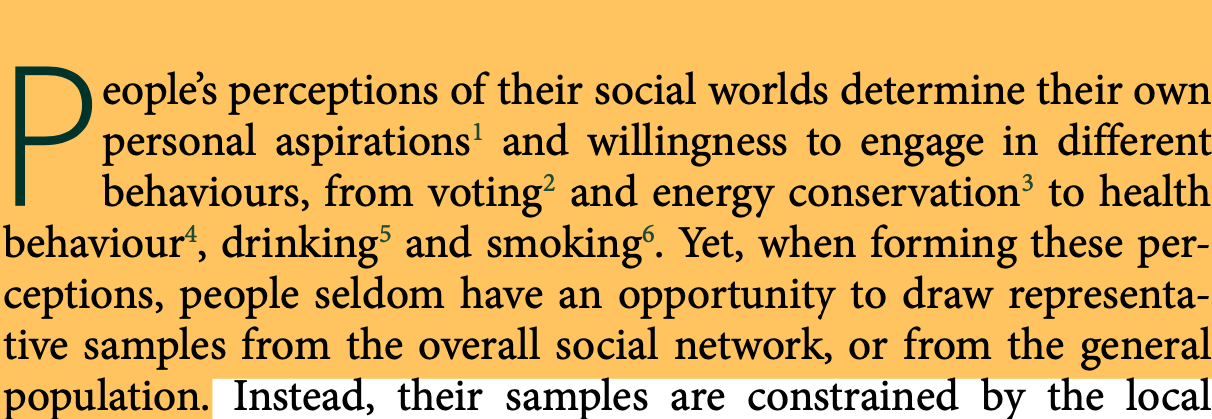
\includegraphics[width=.75\textwidth]{static/perception.png}
    \end{center}
\end{frame}

\begin{frame}
    \begin{center}
        \large{\textsc{What is the effect of different network properties on social perceptions?}}

    \end{center}
\end{frame}


\begin{frame}
    \begin{center}
        
\includegraphics[width=.07\textwidth]{static/search.png} \\ \vspace{.5cm}
        \large{Homophily} \\ \vspace{.5cm}
        \large{Assymetric Homophily} \\ \vspace{.5cm}
        \large{Group Size of the minority}
    \end{center}
\end{frame}

\begin{frame}
    \begin{center}
        
\includegraphics[width=.07\textwidth]{static/toolbox.png} \\ \vspace{.5cm}
        \large{Survey} \\ \vspace{.5cm}
        \large{Network Model} \\ \vspace{.5cm}
        \large{Real World Networks} \\ \vspace{.5cm}
    \end{center}
\end{frame}

\begin{frame}
    \begin{columns}
        \begin{column}{.5\textwidth}
            \begin{center}
                \includestandalone[width=\textwidth]{static/biased}
            \end{center}
        \end{column} \pause
        \begin{column}{.5\textwidth}
            \begin{center}
                $$B_{\text{indv}, i} = \frac{1}{f_m} \frac{\sum_{j \in \Lambda_i} x_j}{k_i}$$
                $$B_{\text{group}} = \frac{1}{|N_g|} \sum_{i \in N_g} B_{\text{indv}, j}$$
                \pause
                $$f_m \approx 0.33$$
                $$ B_{\text{indv}, i} \approx  \frac{0.16}{0.33} \approx 0.5 $$
                \pause
                $$B_{\text{group}} \approx  \frac{0.15}{0.33} \approx 0.45 $$
            \end{center}
        \end{column}
    \end{columns}
\end{frame}

\begin{frame}
    \begin{columns}
        \begin{column}{.5\textwidth}
            \begin{center}
                \includestandalone[width=.75\textwidth]{static/biased}
                $$ B_{\text{indv}, i} \approx \frac{0.16}{0.33} \approx 0.5 $$
                $$B_{\text{group}} \approx  \frac{0.15}{0.33} \approx 0.45 $$
            \end{center}
        \end{column}
        \begin{column}{.5\textwidth}
            \begin{center}
                \includestandalone[width=.75\textwidth]{static/biased_without_homophily}
                $$ B_{\text{indv}, i} \approx  \frac{0.66}{0.33} \approx 2 $$
                $$B_{\text{group}} \approx  \frac{0.52}{0.33} \approx 1.6 $$
            \end{center}
        \end{column}
    \end{columns}
\end{frame}

\begin{frame}
    \centering
    \Large{\textsc{Survey}} \\ \vspace{1cm}
    \begin{columns}
        \begin{column}{.33\textwidth}
            \centering
            
\includegraphics[width=.30\textwidth]{static/germany.png} \\
            $n=99$
        \end{column}
        \begin{column}{.33\textwidth}
            \centering
            
\includegraphics[width=.30\textwidth]{static/south-korea.png} \\
            $n=100$
        \end{column}
        \begin{column}{.33\textwidth}
            \centering
            
\includegraphics[width=.30\textwidth]{static/united-states.png} \\
            $n=101$
        \end{column}
    \end{columns}
\end{frame}

\begin{frame}
\begin{center}
    
\includegraphics[width=.1\textwidth]{static/no-smoke.png}
\includegraphics[width=.1\textwidth]{static/smoke.png}
\end{center}
\pause
\Large
1. Do you smoke? $\rightarrow i$ \\ \pause
2. How many of your friends smoke? $\rightarrow h$ \\ \pause
3. What is the percentage of people in your country who smoke? $\rightarrow \text{perception of } m$ \\
\end{frame}

\begin{frame}
    \begin{center}
        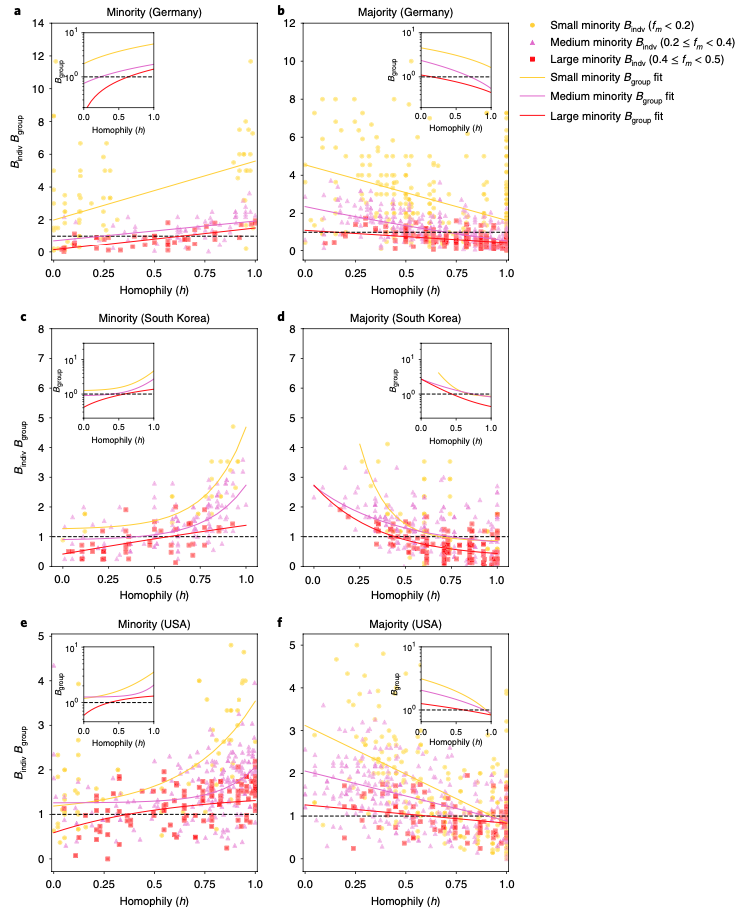
\includegraphics[width=.55\textwidth]{static/survey_results.png}
    \end{center}
\end{frame}

\begin{frame}
    \centering
    \Large{\textsc{Network Model}} \\ \vspace{1cm}
    \pause
    \includestandalone[width=\textwidth]{static/model} 
\end{frame}

\begin{frame}
    \begin{center}
        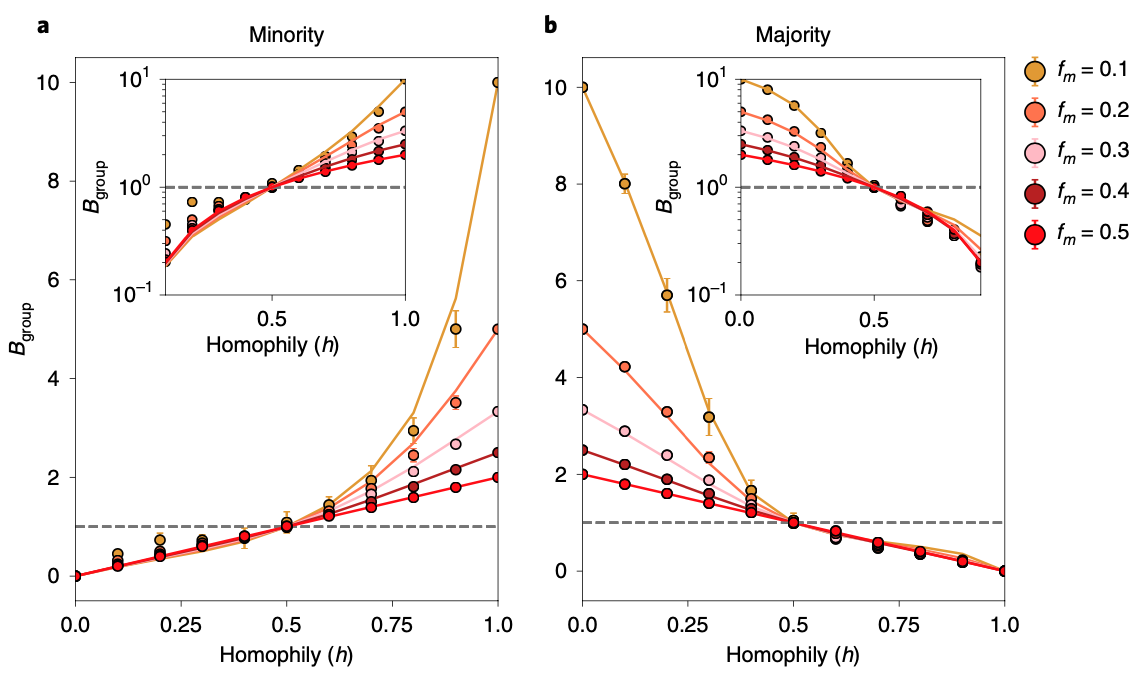
\includegraphics[width=.75\textwidth]{static/model_results.png}
    \end{center}
\end{frame}

\begin{frame}
    \centering
    \Large{\textsc{Real World Networks}} \\ \vspace{1cm}
    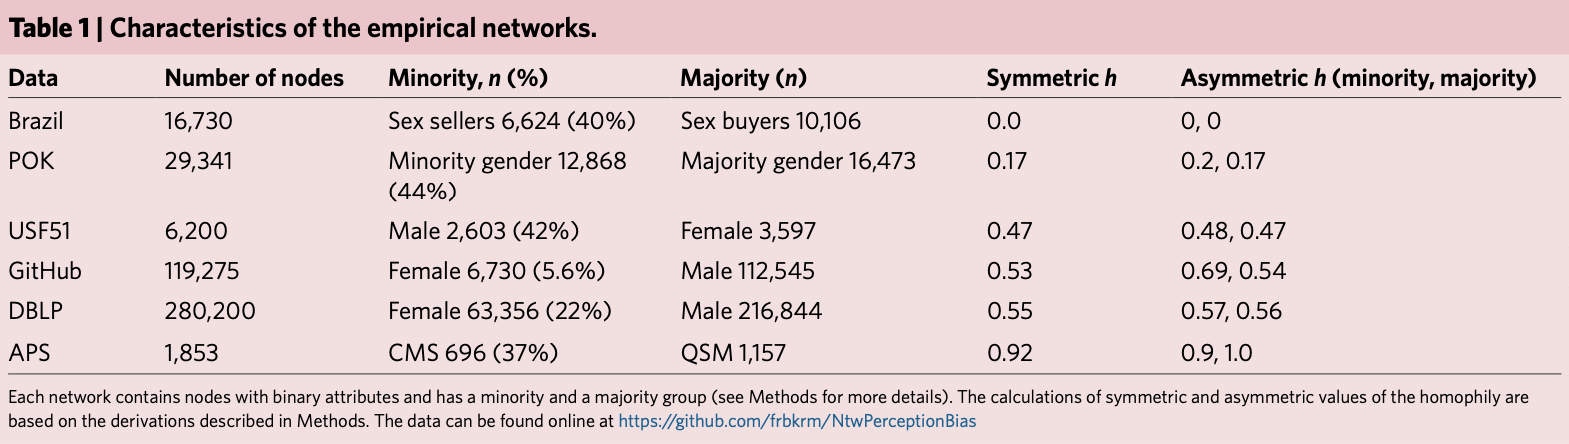
\includegraphics[width=\textwidth]{static/real_world_networks.png}
\end{frame}

\begin{frame}
    \begin{center}
        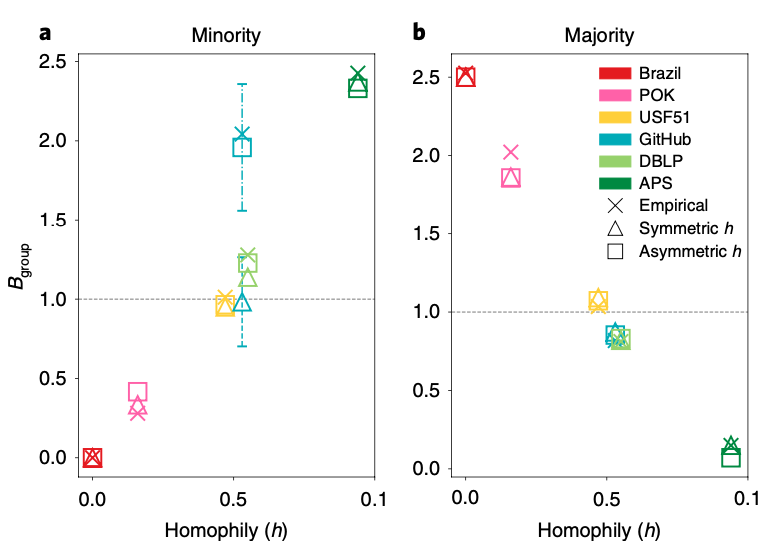
\includegraphics[width=.75\textwidth]{static/real_world_networks_results.png}
    \end{center}
\end{frame}

\begin{frame}
    \centering
    \Large{\textsc{Reducing social perception biases}} \\ \vspace{1cm}
    \includestandalone[width=.35\textwidth]{static/biased}
\end{frame}

\begin{frame}
    \begin{center}
        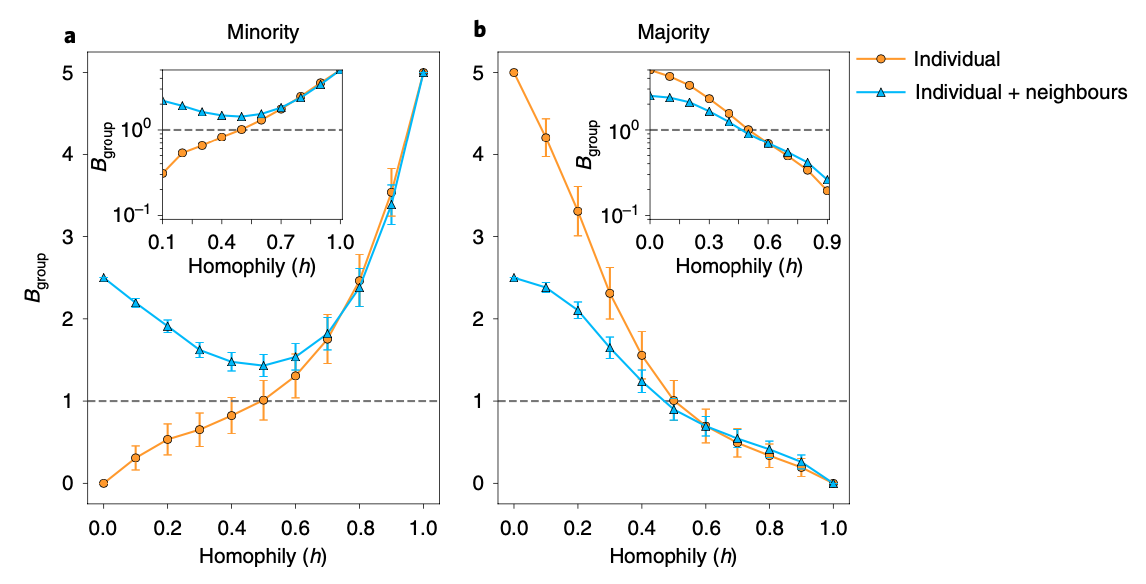
\includegraphics[width=\textwidth]{static/reduce_biase_results.png}
    \end{center}
\end{frame}

\begin{frame}
    \centering
    \Large{\textsc{Summary}} \\ \vspace{1cm}
\end{frame}
\end{document}